\documentclass[a4paper, 12pt, openany]{book}

%%% Работа с русским языком % для pdfLatex
\usepackage{cmap}					% поиск в~PDF
\usepackage{mathtext} 				% русские буквы в~фомулах
\usepackage[T2A]{fontenc}			% кодировка
\usepackage[utf8]{inputenc}			% кодировка исходного текста
\usepackage[english,russian]{babel}	% локализация и переносы
\usepackage{indentfirst} 			% отступ 1 абзаца
\usepackage{gensymb}				% мат символы?

%%% Работа с русским языком % для XeLatex
%\usepackage[english,russian]{babel}   %% загружает пакет многоязыковой вёрстки
%\usepackage{fontspec}      %% подготавливает загрузку шрифтов Open Type, True Type и др.
%\defaultfontfeatures{Ligatures={TeX},Renderer=Basic}  %% свойства шрифтов по умолчанию
%\setmainfont[Ligatures={TeX,Historic}]{Times New Roman} %% задаёт основной шрифт документа
%\setsansfont{Comic Sans MS}                    %% задаёт шрифт без засечек
%\setmonofont{Courier New}
%\usepackage{indentfirst}
%\frenchspacing

%%% Дополнительная работа с математикой
\usepackage{amsfonts,amssymb,amsthm,mathtools}
\usepackage{amsmath}
\usepackage{icomma} % "Умная" запятая: $0,2$ --- число, $0, 2$ --- перечисление
\usepackage{upgreek}

%% Номера формул
%\mathtoolsset{showonlyrefs=true} % Показывать номера только у тех формул, на которые есть \eqref{} в~тексте.

%%% Страница
\usepackage{extsizes} % Возможность сделать 14-й шрифт

%% Шрифты
\usepackage{euscript}	 % Шрифт Евклид
\usepackage{mathrsfs} % Красивый матшрифт

%% Свои команды
\DeclareMathOperator{\sgn}{\mathop{sgn}} % создание новой конанды \sgn (типо как \sin)
\DeclareMathOperator{\rg}{\mathop{rg}}
\DeclareMathOperator{\Rg}{\mathop{Rg}}
\DeclareMathOperator{\im}{\mathop{Im}}
%\DeclareMathOperator{\dim}{\mathop{dim}}
\usepackage{csquotes} % ещё одна штука для цитат
\newcommand{\pd}[2]{\ensuremath{\cfrac{\partial #1}{\partial #2}}} % частная производная
\newcommand{\abs}[1]{\ensuremath{\left|#1\right|}} % модуль
\renewcommand{\phi}{\ensuremath{\varphi}} % греческая фи
\newcommand{\pogk}[1]{\!\left(\cfrac{\sigma_{#1}}{#1}\right)^{\!\!\!2}\!} % для погрешностей

% Ссылки
\usepackage{color} % подключить пакет color
% выбрать цвета
\definecolor{BlueGreen}{RGB}{49,152,255}
\definecolor{Violet}{RGB}{120,80,120}
% назначить цвета при подключении hyperref
\usepackage[unicode, colorlinks, urlcolor=blue, linkcolor=blue, pagecolor=blue, citecolor=blue]{hyperref} %синие ссылки
%\usepackage[unicode, colorlinks, urlcolor=black, linkcolor=black, pagecolor=black, citecolor=black]{hyperref} % для печати (отключить верхний!)


%% Перенос знаков в~формулах (по Львовскому)
\newcommand*{\hm}[1]{#1\nobreak\discretionary{}
	{\hbox{$\mathsurround=0pt #1$}}{}}

%%% Работа с картинками
\usepackage{graphicx}  % Для вставки рисунков
\graphicspath{{images/}{images2/}}  % папки с картинками
\setlength\fboxsep{3pt} % Отступ рамки \fbox{} от рисунка
\setlength\fboxrule{1pt} % Толщина линий рамки \fbox{}
\usepackage{wrapfig} % Обтекание рисунков и таблиц текстом
\usepackage{multicol}

%%% Работа с таблицами
\usepackage{array,tabularx,tabulary,booktabs} % Дополнительная работа с таблицами
\usepackage{longtable}  % Длинные таблицы
\usepackage{multirow} % Слияние строк в~таблице
\usepackage{caption}
\captionsetup{labelsep=period, labelfont=bf}

%%% Оформление
\usepackage{indentfirst} % Красная строка
%\setlength{\parskip}{0.3cm} % отступы между абзацами
%%% Название разделов
\usepackage{titlesec}
\titlelabel{\thetitle.\quad}
\renewcommand{\figurename}{\textbf{Рис.}}		%Чтобы вместо figure под рисунками писал "рис"
\renewcommand{\tablename}{\textbf{Таблица}}		%Чтобы вместо table над таблицами писал Таблица
\usepackage{enumitem}
\setlist{nolistsep}
\usepackage{verbatim}

%%% Теоремы
\theoremstyle{plain} % Это стиль по умолчанию, его можно не переопределять.
\newtheorem{theorem}{Теорема}[section]
\newtheorem{proposition}[theorem]{Утверждение}
\newtheorem{predlog}{Предложение}[section]
\newtheorem{lemma}{Лемма}[section]

\theoremstyle{definition} % "Определение"
\newtheorem{definition}{Определение}[section]
\newtheorem{corollary}{Следствие}[theorem]
\newtheorem{problem}{Задача}[section]

\theoremstyle{remark} % "Примечание"
\newtheorem*{nonum}{Решение}
\newtheorem{zamech}{Замечание}[theorem]

%%% Правильные мат. символы для русского языка
\renewcommand{\epsilon}{\ensuremath{\varepsilon}}
\renewcommand{\phi}{\ensuremath{\varphi}}
\renewcommand{\kappa}{\ensuremath{\varkappa}}
\renewcommand{\le}{\ensuremath{\leqslant}}
\renewcommand{\leq}{\ensuremath{\leqslant}}
\renewcommand{\ge}{\ensuremath{\geqslant}}
\renewcommand{\geq}{\ensuremath{\geqslant}}
\renewcommand{\emptyset}{\varnothing}

%%% Для лекций по инфе
\usepackage{alltt}
\newcounter{infa}[section]
\newcounter{num}
\definecolor{infa}{rgb}{0, 0.2, 0.89}
\definecolor{infa1}{rgb}{0, 0.3, 1}
\definecolor{grey}{rgb}{0.5, 0.5, 0.5}
\newcommand{\tab}{\ \ \ }
\newcommand{\com}[1]{{\color{grey}\##1}}
\newcommand{\num}{\addtocounter{num}{1}\arabic{num}\tab}
\newcommand{\defi}{{\color{infa}def}}
\newcommand{\ini}{{\color{infa}in}}
\newcommand{\rangei}{{\color{infa}range}}
\newcommand{\fori}{{\color{infa}for}}
\newcommand{\ifi}{{\color{infa}if}}
\newcommand{\elsei}{{\color{infa}else}}
\newcommand{\printi}{{\color{infa1}print}}
\newcommand{\maxi}{{\color{infa}max}}
\newcommand{\classi}{{\color{infa}class}}
\newcommand{\returni}{{\color{infa}return}}
\newcommand{\elifi}{{\color{infa}elif}}
\newenvironment{infa}[1]{
	
	\vspace{0.5cm}
	\addtocounter{infa}{1}%
	\noindent{\large \textbf{Программа №\thesection.\arabic{infa}}}\textbf{<<#1>>}%
	\begin{alltt}%
	}{\end{alltt}
	\setcounter{num}{0}
	\vspace{0.1cm}}
%Пример кода:
%\begin{infa}{Поразрядная сортировка}
%	\ \num \defi count_sort(a):\tab \com{определяет нашу функцию}
%	\ \num \tab m = \maxi(a)+1
%	\ \num \tab q = [0]*m
%	\ \num \tab \fori x \ini a:
%	\ \num \tab \tab q[x] += 1
%	\ \num \tab pos = 0
%	\ \num \tab \fori x \ini q:
%	\ \num \tab \tab \fori i \ini \rangei(q[x]):
%	\ \num \tab \tab \tab a[pos] = x
%	\num \tab \tab \tab pos += 1
%\end{infa}

\title{Inf_lections}
\author{Георгий Демьянов}
\date{today}
\usepackage[left=1.27cm,right=1.27cm,top=2cm,bottom=2cm]{geometry}

\usepackage{fancyhdr} % Для колонтитулов

\renewcommand{\baselinestretch}{1.3}

\makeatletter % Убирает нумерацию на страницах, где \chapter
\renewcommand\chapter{\if@openright\cleardoublepage\else\clearpage\fi
	\thispagestyle{empty}% original style: plain
	\global\@topnum\z@
	\@afterindentfalse
	\secdef\@chapter\@schapter}
\makeatother


\begin{document}
%\thispagestyle{empty}
\def\chaptername{ЛЕКЦИЯ} % Семинар вместо главы
\setcounter{tocdepth}{1} % Глубина отображения в оглавлении

\begin{titlepage}
	\begin{center}
		{\large Московский физико--технический институт}
		\vfill
		\vfill
		{\Large \textbf{Т.Ф. ХИРЬЯНОВ}}
		\vspace{1.5cm}
		
		
		{\textbf{{\Huge ЛЕКЦИИ\\\smallskip ПО ИНФОРМАТИКЕ}\\ \Large Весенний семестр,\\ 2016--2017 учебный год}}
		\bigskip
	\end{center}
	\vfill
	
	\hfill\begin{minipage}{0.4\textwidth}
		{\centering
				При поддержке:\\
				Г. Демьянов, \href{https://vk.com/id37346992}{VK}\\
				С. Клявинек, \href{https://vk.com/id85132547}{VK}\\
				Отдельная благодарность:\\
				<<Полиция КПМ>>: А. Кожарин, \href{https://vk.com/id92540660}{VK}\\	
			}
	\end{minipage}%

	\vfill
	\begin{center}
		Москва, 2017 г.
	\end{center}
\end{titlepage}

\fancypagestyle{plain1}{ %
	\fancyhead{} % remove everything
	\fancyfoot{}
	\renewcommand{\headrulewidth}{0.5pt}
	%\renewcommand{\footrulewidth}{0pt}
	%\fancyhead[RO, RE]{\textbf{\large \thepage}} 
	%\fancyhead[CE, CO]{\hrule\smallskip{\small \text{\rightmark}}}% odd-center, with the name of the Section
	\fancyhead[CE, CO]{ОГЛАВЛЕНИЕ}% Even-center, with the name of the Chapter.
	%\fancyfoot[L,R,C]{}
	\fancyhead[R]{\hrule\smallskip\textbf{\large \thepage}}
}
\pagestyle{plain1}
{
\tableofcontents
}

\newpage % НЕ УБИРАТЬ, ПОЛОМАЕТСЯ!!!

\fancypagestyle{plain}{ %
	\fancyhead{} % remove everything
	\renewcommand{\headrulewidth}{0.5pt}
	\renewcommand{\footrulewidth}{0pt}
	\fancyhead[RO, RE]{\textbf{\large \thepage}} 
	\fancyhead[CE]{\hrule\smallskip{\small \text{\rightmark}}}% odd-center, with the name of the Section
	\fancyhead[CO]{\hrule\smallskip ЛЕКЦИЯ \thechapter}% Even-center, with the name of the Chapter.
	\fancyfoot[L,R,C]{}
	%\fancyhead[C]{\normalsize\thepage}
}
\pagestyle{plain}

\chapter{Повторение}
\section{Ссылочная модель данных}
Ссылочная модель данных - объекты существуют независимо от времен.
\begin{alltt}
>>> 2+3
5
\end{alltt}
Создаются два объекта типа int.
\begin{alltt}
2.__add__(3) - метод добавления
\end{alltt}
\begin{alltt}
	x = 2+3 # x ссылается на объект 5
	x = 'Hello' # возникает объект строки
\end{alltt}
После вывода результата объекты 2, 3, 5 удаляются, т.к. нет ссылки на эти объекты.
Если x перестал ссылаться на 5, объект 5 уничтожается.
\begin{alltt}
x = 5
y = x
x = 'Hello'
y = None
\end{alltt}
После того, как y начал ссылаться на None, объект 5 уничтожается.
\begin{alltt}
	x = (2+3+5)**5**5 # приоритет у возведения в степени
\end{alltt}

Т.е. в начале выполняется 5**5, а потом (2+3+5)**25.

Начиная с версии Python 3.6, можно разделять числа так:
\begin{alltt}
x = 100_001
y = 0xAF_DC
\end{alltt}
\section{Пространство имен}
4 пространства: локальные, окружающие, глобальные, строенные (LEGB).

y = 10*x+7
Сначала будет происходить поиск локального x, затем в надпространстве, затем в глобальных, в последнюю очередь - во встроенных переменных.

Если написать 
max = 10,
то функция max перестанет работать.

Пример:
\begin{infa}{}
\num \defi f(A):
\num \tab A = A + 10 \com{если написать A += 10 ошибки не будет}
\num B = [1, 2, 3]
\num f(B)
\num \printi(*B) \com{1 2 3}
\end{infa}

Строки и числа --- неизменяемые объекты.
f является именем объекта functional.

def --- по сути это операция создания нового объекта.

Любой вызов функции порождает свое пространство имен, которое перестанет существовать после выполнения return. 

A начинает ссылаться на [1, 2, 3]. После конкатинации A начинает ссылаться на [1, 2, 3, 4]. A ссылается на глобальный объект, и начинает ссылаться на локальный объект. После return уничтожается A и список [1, 2, 3, 4].

Или можно записать так:
\begin{infa}{}
	\num \defi f(A):
	\num \tab A.append(10)
	\num B = [1, 2, 3]
	\num f(B)
	\num \printi(*B) \com{1 2 3}
\end{infa}

Функция должна что-то возвращать. В частном случае, можно возвращать несколько параметров. Нарушить ссылочную модель можно только "залезая"\ в глобальные имена.

\begin{infa}{}
	\num d=1
	\num \defi f(A):
	\num \tab \globali d
	\num \tab A.append(d)
	\num \tab d = d + 1
\end{infa}







\section{ООП}
Тип тоже является объектом типа тип. 
\begin{infa}{}
\num \classi Base:
\num \tab x = 10
\num \tab \defi g(self, x0):
\num \tab \tab self.x = x0
\num b = Base()
\num \printi(b.x)
\end{infa}

\begin{infa}{}
	\num \classi Base:
	\num \tab x = 10
	\num \tab \defi g(self, x0)
	\num \tab \tab self.x += x0
	\num b = Base()
	\num \printi(b.x)
\end{infa}

Нужно создавать атрибуты только в методе init!

\section{Элементы функционального программирования}

\subsection{Функция map}
\begin{alltt}
x, y, z = map(int, input().split()) \com{считывание трех чисел с клавиатуры}
\end{alltt}

Функция map применяет к каждому объекту функцию, которую мы написали. В нее же можно написать свою функцию:
\begin{alltt}
x, y, z = map(lambda x: int(x)**2, input().split())
	A == list(map(int, range(100)))
	B = map(float, int(x) for x in input().split())
\end{alltt}

map возвращает объект типа map.

\subsection{Применение lambda-функций}
$x^2+e^{1/x}+\ln x$
\begin{alltt}
x = decompoused_value # нужно объявлять функцию
(lambda x: x**2 + exp(1/x)+ln(x))(2) #хороший пример использования lambda
\end{alltt}

\subsection{Функция enumerate}
\begin{infa}{}
\num A = [10, 20, 30]
\num \fori i,x \ini \enumeratei(A): \com{А используется как итерируемый объект}
\num \tab \printi(i,x) \com{(0,10), (1,20), (2,30) - эту конструкцию нам вернет enumerate(A)}
\num \tab x = x + 1	\com{Значение в массиве не изменилось, мы только испортили х}
\end{infa}
\subsection{Функция zip}

\begin{alltt}
A = [1, 2, 3, 4, 5]
B = 'Hello'
c = list(zip(A,B)) \com{результат есть zip-object}
\end{alltt} 
\chapter{Графы}
\section{Графы}
Граф --- множество вершин и инцедентных им ребер.
$$G=(V, E)$$
$$v \in V, \qquad e \in E $$
Говорят, что ребро $e$ инцедентно вершине $v$, если она является его концом.

Допустимы графы:
$$G = (\varnothing, \varnothing)$$
$$G = ({1}, \varnothing)$$
Недопустим граф:
$$G = (\varnothing, {a})$$

Граф --- "упрощенная модель".

У ребра \underline{2 конца}. Это не обязательно отрезок. 

Ребро может быть петлей.

2 разных ребра могут быть инцедентно двум вершинам --- кратные ребра.

У классического графа 2 конца. Но может быть ориентированный граф. Т.е. либо у ребра 2 конца, либо у него есть начало и конец. Тогда ребро называется дуга. Короткое название \textbf{орграф}.

\section{Задача Эйлера о семи кёнигсбергских мостах}
Как пройти по всем городским мостам (через реку Преголя), не проходя ни по одному из них дважды?
\begin{figure}[h!]
	\noindent\centering{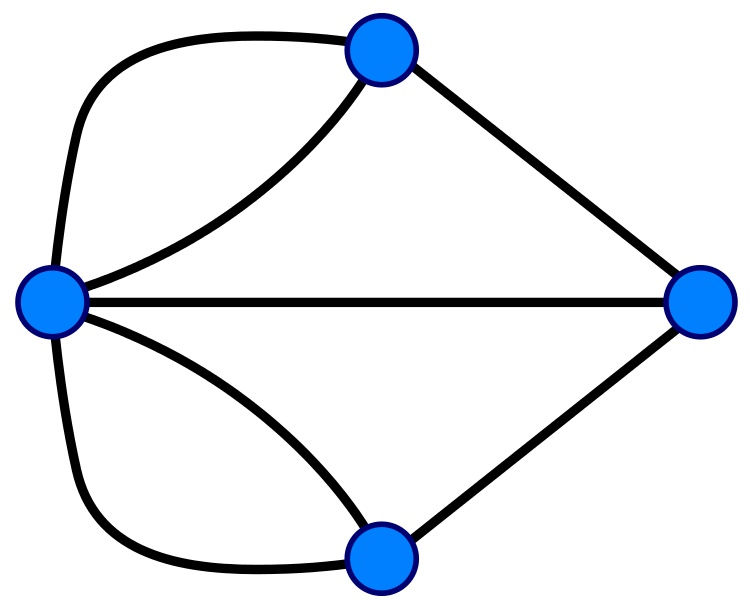
\includegraphics[width=8cm]{lection_17/graph.jpg}}
	\caption{Граф к задаче о мостах}
	\label{fp_2}
	\vspace{-0.5cm}
\end{figure}

\textit{Введем дополнительные понятия:}

Степень вершины --- количество инцедентных ей ребер.

Граф G' = (V', E') является подграфом G, если V' $\subset$ V, E' $\subset$ E.

Путь --- последовательность ребер (в которой конец каждого ребра есть начало следующего).

Путь тоже является графом, а точнее это орграф, подграф исходного.

Любой неориентированный граф можно представить как ориентированный.

Цикл --- путь, в котором начало пути (начало первого ребра) совпадает с концом (конец последнего ребра).

Рассмотрим граф A---B.

Возможны пути
$$[AB, BA]$$

Простой путь --- путь, у которого не повторяются ребра (вершины повторятся могут).

Простой цикл ---  цикл, у которого не повторяются ребра (вершины повторятся могут).

\textbf{Вернемся к задаче.}

Пусть вершина верхняя вершина --- старт. Пройдем по ребру и выкинем его (т.е. степень у вершины понизится). Продолжим процесс аналогично. В итоге какой бы путь мы не строили, степени у всех промежуточных вершин понизятся на четное число, а у вершин финиша и начала понизятся на нечетное число. Т.о. это невозможно. Подробнее \href{https://ru.wikipedia.org/wiki/%D0%97%D0%B0%D0%B4%D0%B0%D1%87%D0%B0_%D0%BE_%D1%81%D0%B5%D0%BC%D0%B8_%D0%BA%D1%91%D0%BD%D0%B8%D0%B3%D1%81%D0%B1%D0%B5%D1%80%D0%B3%D1%81%D0%BA%D0%B8%D1%85_%D0%BC%D0%BE%D1%81%D1%82%D0%B0%D1%85}{в вики}.

Эйлеров цикл --- простой цикл, включающий все ребра графа.

Эйлеров граф --- граф, в котором существует Эйлеров цикл.

Полуйэлеров граф --- граф, в котором есть Эйлеров путь, но нет Эйлерого цикла.

\section{Связность графов}
Граф является связным, если для $\forall A,B \in V$ существует путь от $A$ к $B$.\\
$A\longrightarrow B\longrightarrow C$ --- несвязный граф.

Компонента связности --- связный подграф, в который включены все вершины исходного, связаные с принадлежащими подграфами. Связный граф имеет 1 компоненту связности. Крайний случай: вершины без ребер. Количество компонент связности от 1 до количества вершин.

Слабая связность графа --- "забываем"\  про направленность графов и смотрим на связность.

Сильно связный граф --- граф связан при условии направленности.

"Вес"\  ребра --- некоторая числовая характеристика ребра (расстояние, время прохождения, стоимость, энергия реакции и т.д.). Это необязательно положительное число.

Взвешенный граф --- граф, у которого все ребра имеют вес.

\section{Хранение графа в памяти ПК}
Введем понятие: смежные вершины --- <<соседи>>, т.е. это вершины, которые имеют общее ребро. Ациклический граф --- орграф без цикла.

\subsection{Формы хранения}
Есть 3 основные формы хранения:\\
1. Список ребер (множество ребер)
\begin{center}
AB 5\\
BC 3\\
CD 1\\
DE 2\\
\end{center}
2. Матрица смежности\\
Матрица смежности не умеет хранить кратные ребра (если только массив не трехмерный (но это бред)).

\begin{center}
\begin{tabular}{|c|c|c|c|c|c|}
	\hline 
	& A & B & C & D & E \\ 
	\hline 
	A & x & 1 & 0 & 0 & 0 \\ 
	\hline 
	B & 1 & x & 1 & 0 & 0 \\ 
	\hline 
	C & 0 & 1 & x & 1 & 0 \\ 
	\hline 
	D & 0 & 0 & 1 & x & 1 \\ 
	\hline 
	E & 0 & 0 & 0 & 1 & x \\ 
	\hline 
\end{tabular}
\end{center}

Можно  также составить матрицу взвешенности, если записать в эту матрицу вес каждого ребра.

\noindent3. Списки смежности\\
\begin{align*}
&A : B\\
&B : A, \quad C\\
&C : B, \quad D\\
&D : C, \quad E\\
&E : D\\
\end{align*}

\subsection{Реализация на Python}
\begin{enumerate}
	\item Список ребер
\begin{infa}{}
\num G = ('AB', 5),
\num \tab ('BC', 3),
\num \tab ('CD', 1),
\num \tab ('DE', 2)
\end{infa}
Но кортежами не очень удобно.
\begin{infa}{}
\num G = {'AB' : 5
\num \tab 'BC' : 3
\num \tab 'CD' : 1
\num \tab 'DE': 2}
\end{infa}

Задачи:
\begin{enumerate}
\item Проверка смежности.
\item Перебор "соседей".
\end{enumerate}

\item Таблица смежности
\begin{infa}{}
\num G = [[0,1,0,0,0],
\num \tab [1,0,1,0,0],
\num \tab [0,1,0,1,0],
\num \tab [0,0,1,0,1],
\num \tab [0,0,0,1,0]]
\end{infa}
Решение задач:
\begin{enumerate}
\item Проверка смежностей
\begin{infa}{}
G[i][k] == 1\text{ - значит смежные}
\end{infa}

\item Перебор соседей: нужно пробежать по строке.
\end{enumerate}

\item Списки смежности

Словарь множеств смежностей:
\begin{infa}{}
\num G = \{'A':\{'B':5\}
\num \tab 'B':\{'A':5, 'C':3\}
\num \tab 'C': \{'B':3, 'D':1\}
\num \tab 'D': \{'C':1, 'E':2\}
\num \tab 'E': \{'D':2\}\}
\end{infa}
Проверка факта смежностей:
\begin{alltt}
	'B' in G['A'] \com{O(1)}
\end{alltt}

Перебор соседей:
\begin{alltt}
for v in G['A']:
\end{alltt}
$O(N_{e_{max}})$, $N_e$ - средняя степень вершины.

\end{enumerate}
\chapter{Обход графа в глубину}
\section{Множества и словари}
\noindent Задание множеств:
\begin{infanoname}
A = None \com{Пустое множество}
A = \{1, 2 'hello'\} \com{Явное перечисление элементов}
A = \seti('hello') \com{Множество букв в строке}
B = [1, 2, 1, 2]; A = \seti(B) \com{Множество из списка или любого итерируемого объекта}
\end{infanoname}
Работа с элементами множеств:
\begin{infanoname}
C = \{1, 2, 'hello'\}
\fori elem \ini \rangei(C): \com{Перебираем все элементы множества}
\tab \printi(elem)
sorted(C) \com{Список из отсортированных элементов множества}
1 \ini C \com{Проверка принадлежности}
2 \noti \ini C
A.add(3) \com{Добавление элемента}
A.remove(3) \com{Удаление элемента, который есть в множестве}
A.discard(4) \com{Удаление элемента, которого может и не быть в множестве}
A.pop() \com{Извлечение случайного элемента из множества с удалением его}
\end{infanoname}
Задание словарей
\begin{infanoname}
D = \{\} \com{Пустой словарь}
D = \{1: 'a', 2: 'b'\} \com{Явное перечисление}
D = \dicti([(1, 'a'), (2, 'b')]) \com{Словарь из списка пар элементов}
D = \dicti(\zipi([1, 2], ['a', 'b'])) \com{Словарь из итерируемого объекта, возвращающего пары\\ значений}
D = \{i: \chri(i + \ordi('a')) \fori i \ini \rangei(1, 3)\} \com{Генератор словарей}
\end{infanoname}
Работа с элементами словаря
\begin{infanoname}
\leni(D) \com{Количество элементов в словаре}
D[key] \com{Поиск по ключу, который есть в словаре}
key in D \com{Проверка принадлежности словарю}
D[key] = value \com{Установка или изменение значения}
\deli D[key] \com{Удаление ключа, который есть в словаре}
value = D.pop(key) \com{Удаление ключа вместе с возвращением значения}
value = D.pop(key, no_key_value)
key, value = D.popitem() \com{Извлечение из словаря пары (ключ, значение) с удалением ключа}
D.get(key, no_key_value) \com{Значение по ключу, no_key_value, если ключа нет}
D[key] = D.get(key, 0) + 1 \com{Самая простая реализация счетчика}
\fori key \ini D: \com{Перебираем все ключи}
\tab \printi(key, D[key])
\fori key, value \ini D.items(): \com{Перебираем все пары (ключ, значение)}
\tab \printi(kay, value)
\fori value \ini D.values(): \com{Перебор всех значений}
\tab \printi(value)
\sortedi(D) \com{Отсортированный список ключей}
\sortedi(D.values()) \com{Отсортированный список значений}
\sortedi(D.items()) \com{Отсортированный по ключу список пар (ключ, значение}
\sortedi(D.items(), \keyi = \lambdai x: x[1])
\end{infanoname}


\section{Реализация записи графа}
\begin{wrapfigure}{r}{0.25\linewidth}
		\begin{center}
			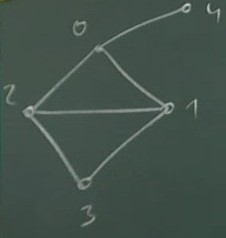
\includegraphics[width=\linewidth]{lection_18/graph1}
			\caption{Пример графа}
			\label{Fig:graph1}
		\end{center}
\end{wrapfigure}
Будем задавать граф как список ребер. Количество вершин, потом количество ребер.\\
$$5\ 6$$
После зададим ребра:
\begin{center}
0 1\\
0 2\\
1 2\\
1 3\\
2 3\\
0 4\\
\end{center}
\begin{infa}{Считывание графа как матрицы и как списка смежностей}
\ \num \defi read_graph_as_matrix():
\ \num \tab N, M = [\inti(x) \fori x \ini \inputi().split()]
\ \num \tab graph = [[0]*N \fori i \ini \rangei(N)] \com{матрица смежностей}
\ \num \tab \fori edge \ini \rangei(M):
\ \num \tab \tab a, b = [\inti(x) \fori x \ini \inputi().split()]
\ \num \tab \tab graph[a][b] = 1
\ \num \tab \tab graph[b][a] = 1
\ \num \tab \returni graph
\ \num
\num \defi print2d(A):
\num \tab \fori line \ini A:
\num \tab \tab print(*line)
\num \tab \printi()
\num
\num \defi read_graph_as_lists():
\num \tab N, M = [\inti(x) \fori x \ini \inputi().split()]
\num \tab graph = [[] \fori i \ini \rangei(N)]
\num \tab \fori edge \ini \rangei(M):
\num \tab \tab a, b = [\inti(x) \fori x \ini \inputi().split()]
\num \tab \tab graph[a].append(b)
\num \tab \tab graph[b].append(a) \com{Для ориентированного графа строка не нужна}
\num \tab \returni graph
\num
\num graph = read_graph_as_lists()
\num print2d(graph)
\end{infa}
В итоге $\texttt{read\_graph\_as\_matrix()}$ даст нам такой результат:
\begin{center}
\vspace{-1cm}
$$
\begin{matrix}
	0&1&1&0&1\\
	1&0&1&1&0\\
	1&1&0&1&0\\
	0&1&1&0&0\\
	1&0&0&0&0\\
\end{matrix}
$$
\end{center}
а $\texttt{read\_graph\_as\_lists()}$:
$$
\begin{matrix}
1&2&4\\
0&2&3\\
0&1&3\\
1&2& \\
0& & \\
\end{matrix}
$$
\section{Алгоритм обхода графа в глубину}
\subsection{Алгоритм}
Перебираем соседей по часовой стрелке. Граф считаем неориентированным.

\textbf{Основное правило: для того, чтобы пойти на праздник надо вначале позвать всех своих друзей на праздник, но только тех, кто еще не позван.}

\begin{figure}[h!]
	\centering
	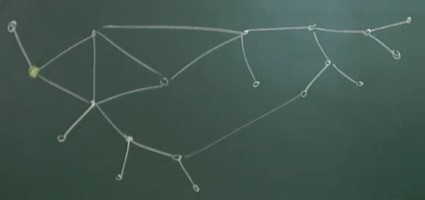
\includegraphics[width=0.5\linewidth]{lection_18/alg1}
	\caption{Граф с выбранным началом}
\end{figure}
Далее по часовой стрелке от 12 часов выбираем следующую вершину и зовём ее на праздник. Будем отмечать порядок обхода (номера показывают не индексы в графе, а просто порядок вызова).

\begin{figure}[h!]
	\centering
	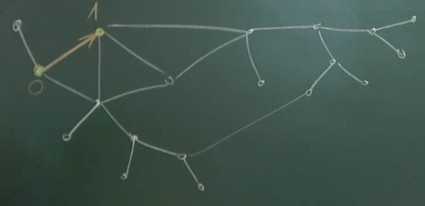
\includegraphics[width=0.5\linewidth]{lection_18/alg2}
	\caption{Точка 1 перекрашена в "серый"\ цвет}
\end{figure}

Теперь вершину 1 красим в "серый"\ цвет. 0-ой ждёт ответа от 1-го.

1-ый начинает перебирать всех своих не позванных соседей по часовой стрелке от 12 часов.
\vspace{10cm}

\begin{figure}[h!]
	\centering
	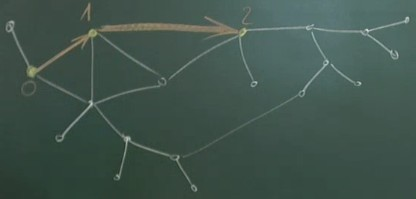
\includegraphics[width=0.5\linewidth]{lection_18/alg3}
	\caption{Точка 2 перекрашена в "серый"\ цвет}
\end{figure}

И так процесс продолжается.
\begin{figure}[h!]
	\centering
	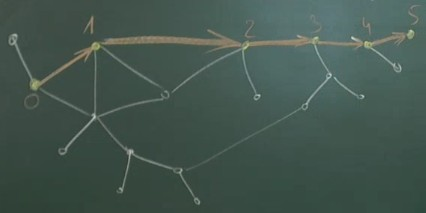
\includegraphics[width=0.5\linewidth]{lection_18/alg4}
	\caption{Точки 0-5 перекрашены в "серый"\ цвет}
\end{figure}

Теперь 5-ый перебирает всех своих соседей. Но у него только один сосед --- это 4-ый, и он уже позван. Т.о. 5-ый уже всех позвал. 5-я точка перекрашивается в "чёрный"\ цвет и идёт на праздник. 4-му возвращается от 5-го команда, что 5-ый всех позвал. Дальше 4-ый продолжает звать друзей и зовёт 6-го. 6-ая точка перекрашивается в "серый"\ цвет.

6-ой перебирает всех друзей и убеждается, что он всех позвал. Точка перекрашивается в "чёрный"\ цвет и идёт на праздник. 4-му возвращается команда, что 6-ой позвал всех друзей.

Т.о. 4-ый тоже позвал всех друзей. Точка перекрашивается в "чёрный"\ и дает команду 3-ему.

\begin{figure}[h!]
	\centering
	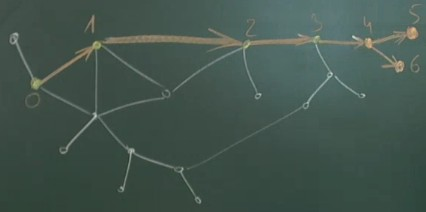
\includegraphics[width=0.5\linewidth]{lection_18/alg5}
	\caption{Точка 4 перекрашена в "чёрный"\ цвет}
\end{figure}

3-ий зовёт оставшихся.

Процесс повторяется...
\vspace{10cm}
\begin{figure}[h!]
	\centering
	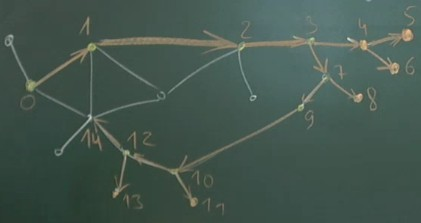
\includegraphics[width=0.5\linewidth]{lection_18/alg6}
	\caption{Дошли до 14}
\end{figure}

14-ый позвал бы 1-го, но он уже позван. Заметим, что из серой вершины мы пытаемся позвать серую вершину, что значит, что в графе есть цикл.

Т.о. 14-ый зовёт следующего по часовой стрелке. 15 точка перекрашивается в "серый". 15-му звать некого, поэтому точка перекрашивается в "чёрный"\ и дает сигнал 14-му.

\begin{figure}[h!]
	\centering
	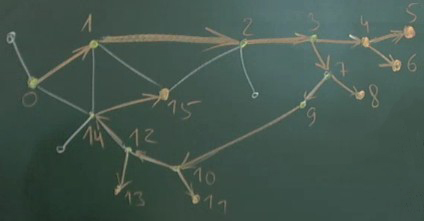
\includegraphics[width=0.5\linewidth]{lection_18/alg7}
	\caption{Прошли 15-го}
\end{figure}

14-ый продолжает звать друзей, зовёт 16-го, 16-ый возвращает сигнал 14-му.

14-му становится некого звать. Он возвращает сигнал 13-му и перекрашивается в "чёрный". 13 возвращает сигнал 12-му и т.д. до 2-го и все они идут на праздник.

\begin{figure}[h!]
	\centering
	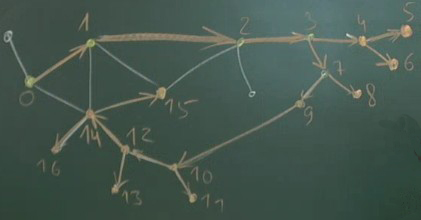
\includegraphics[width=0.5\linewidth]{lection_18/alg8}
	\caption{Длинный возврат}
\end{figure}

2-ой зовёт 17-го, ему в свою очередь звать некого, он идёт на праздник и возвращает сигнал 2-му. 2-ой тоже всех позвал. В итоге сигнал возвращается 0-му, который зовёт 18-го. В итоге, все точки перекрашены в "чёрный"\ цвет. 

\begin{figure}[h!]
	\centering
	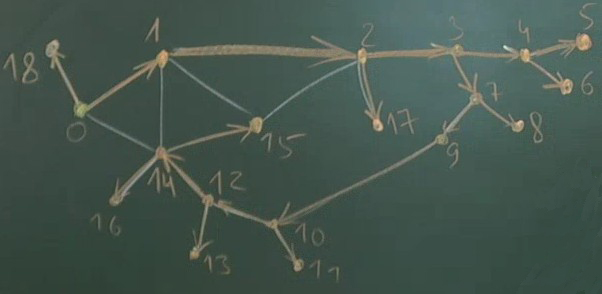
\includegraphics[width=0.5\linewidth]{lection_18/alg9}
	\caption{Все позваны}
\end{figure}

Применение обхода в глубину:
\begin{enumerate}
	\item Проверка связности графа (будем добавлять вершины в множество пройденых вершин)
	\item Выделение компонентов связности
	\item Поиск циклов (проверка ацикличности графов)
	\item Поиск компонент сильной связности орграфов (алгоритм Косарайю)
\end{enumerate}

\subsection{Реализация на Python}

\begin{infa}{Построение алгоритма}
\ \num \defi read_graph_as_lists():
\ \num \tab N, M = [\inti(x) \fori x \ini \inputi().split()]
\ \num \tab graph = [[] \fori i \ini \rangei(N)]
\ \num \tab \fori edge \ini \rangei(M):
\ \num \tab \tab a, b = [\inti(x) \fori x \ini \inputi().split()]
\ \num \tab \tab graph[a].append(b)
\ \num \tab \tab graph[b].append(a)
\ \num \tab \returni graph
\ \num 
\num \defi call_all_friends(me, friends, already_called = \Nonei):
\num \tab \ifi already_called \isi \Nonei:
\num \tab \tab already_called = \seti()
\num \tab {\color{grey}""" Правило: тебя позвали на праздник, но пойти можно только тогда, когда\\ \phantom{12 \tab \tab """}позовешь всех своих еще не позванных друзей \\\phantom{12 \tab \tab}"""}
\num \tab already_called.add(me)
\num \tab \fori friend \ini friends[me]:
\num \tab \tab \ifi friend \noti \ini already_called:
\num \tab \tab \tab \printi(friend, 'был позван на праздник')
\num \tab \tab \tab call_all_friends(friend, friends, already_called)
\num \tab \tab \tab \printi(friend, 'пошел на праздник')
\num
\num graph = read_graph_as_lists()
\num call_all_frineds(0, graph)
\end{infa}
Запишем теперь более строго:
\begin{infa}{Реализация алгоритма обхода графа в глубину}
\ \num \defi dfs(vertex, graph, used = \Nonei): \com{Depth-first search}
\ \num \tab \ifi used \isi \Nonei:
\ \num \tab \tab used = \seti()
\ \num \tab used.add(vertex)
\ \num \tab \fori neighbour \ini graph[vertex]:
\ \num \tab \tab \ifi neighbour \noti \ini used:
\ \num \tab \tab \tab dfs(neighbour, graph, used) 
\ \num
\ \num graph = read_graph_as_lists()
\num used = \seti()
\num number_of_components = 0
\num \fori vertex \ini \rangei(\leni(graph)): \com{Подсчет компонент связности}
\num \tab \ifi vertex \noti \ini used:
\num \tab \tab dfs(vertex, graph, used)
\num \tab \tab number_of_components += 1
\num
\num \printi('Количество компонент связности:', number_of_components)
\end{infa}
\section{Дерево}
Дерево --- связный граф, в котором
\begin{enumerate}
	\item Нет простых циклов
	\item От a к b только один путь
	\item $N_{\text{вершин}}=M_{\text{ребер}}+1$
\end{enumerate}

Ориентированное дерево --- ациклический орграф, в котором только одна вершина имеет нулевую степень захода (корень).
Вершины с нулевой степенью исхода называются "листья". Остальные --- узлы ветвления. Для корневого дерева можно ввести уровень узла --- длина пути от корня до вершины (уровень иерархии).

У любого связного графа есть подграф, являющийся деревом и содержащий все исходные вершины.

Вершина сама по себе тоже является деревом.

Остовное дерево --- пограф исходного графа, в котором выброшено максимальное количество ребер так, чтобы связность еще сохранилась. Обход графа в глубину позволяет построить одно из остовных деревьев.

Свойства:
\begin{itemize}
	\item Дерево не имеет кратных ребер и петель
	\item Граф является деревом $\Leftrightarrow$ когда любые две различные вершины можно соединить  единственным простым путем (простой цепью).
	\item Любое дерево однозначно определяется расстояниями между его концевыми вершинами со степенью 1 (длиной наименьшей цепи).
	\item Любое дерево, множество вершин которого более чем счетное является планарным графом.
\end{itemize}

Шарнир --- вершина, при удалении которой количество компонент связности увеличивается.

\begin{wrapfigure}{r}{0.2\linewidth}
	\begin{center}
		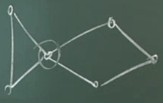
\includegraphics[width=\linewidth]{lection_18/sharnir}
		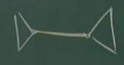
\includegraphics[width=\linewidth]{lection_18/most}
		\caption{Шарнир и мост}
		\label{Fig:sharnir}
		\vspace{-4cm}
	\end{center}
\end{wrapfigure}

Мост --- ребро, при удалении которого количество компонент связности увеличивается. Такие ребра еще известны как разрезающие ребра или перешейки.

У дерева любая вершина является шарниром, а любое ребро мостом.


\section{Алгоритм Косарайю}
Задача: поиск сильно связной компоненты орграфа. Возьмем такой орграф. В нем будет 1 слабая компонента.
\vspace{1.2cm}
\begin{figure}[h!]
	\centering
	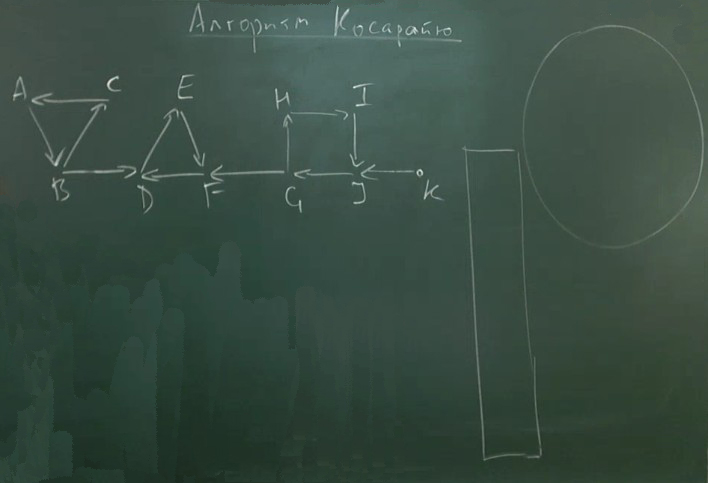
\includegraphics[width=0.8\linewidth]{lection_18/kos1}
	\caption{Орграф}
\end{figure}

Запустим обход в глубину. Пусть будет множество вершин, которых мы уже использовали, и список вершин в порядке обхода (типа как стек).

Начнем с вершины A. Из A вызываем B. Они оказываются в множестве использованных вершин, также заполняется стек вызванных вершин. Далее вызовем вершину D (не принципиально D или C), добавим ее в множество и стек аналогично. Далее вызовем E, потом F. После происходит откат, и мы вызываем вершину C. Дальше выбираем любую вершину, которую не использовали. Пусть это будет G. Потом вызываем H, I, J. Остается вершина K, она становится последней.
\vspace{10cm}
\begin{figure}[h!]
	\centering
	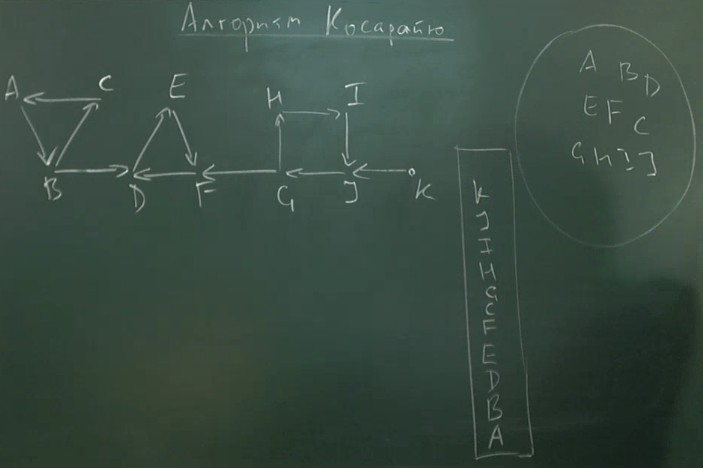
\includegraphics[width=0.8\linewidth]{lection_18/kos2}
	\caption{После прохождения по графу}
\end{figure}

Далее мы разворачиваем наш граф, т.е. меняем все направления. А теперь от верхней вершины в стеке запустим обход в глубину на обращенном графе.

\begin{figure}[h!]
	\centering
	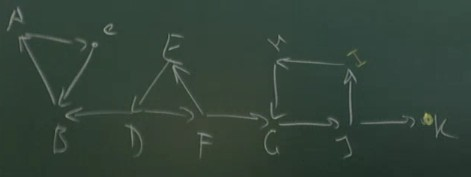
\includegraphics[width=0.5\linewidth]{lection_18/kos3}
	\caption{Обращенный граф}
\end{figure}

Но от K дойти никуда нельзя. Это и есть сильная компонента. K добавляем в новое множество использованных вершин. 

Дальше начинаем обход с вершины I, т.е. I--->H--->G--->J. Их добавляем в множество использованных и стираем из стека. Дальше идти опять некуда. Значит, это вторая сильная компонента.

Переходим к вершине C. Выполняем обход: C--->B--->A. Их добавляем в множество использованных и стираем из стека. Дальше идти некуда. Т.о. это еще одна компонента сильной связности.

Переходим к вершине F. В G уже не идем т.к. она использована. Выполняем обход F--->E--->D. Их добавляем в множество использованных и стираем из стека. Дальше идти некуда. Т.о. это еще одна компонента сильной связности.

В итоге получилось 4 компонент сильной связности.

Примечание: не принципиально, оборачивать ли граф сначала или потом (по \href{https://ru.wikipedia.org/wiki/%D0%90%D0%BB%D0%B3%D0%BE%D1%80%D0%B8%D1%82%D0%BC_%D0%9A%D0%BE%D1%81%D0%B0%D1%80%D0%B0%D0%B9%D1%8E}{википедии} сначала нужно развернуть граф).
\chapter{Обход графа в ширину (BFS)}
\section{Визуализация алгоритма BFS (пожар на графе)}
\begin{wrapfigure}{r}{0.4\linewidth}
\begin{frame}{Анимация BFS}
	\animategraphics[loop,controls,width=\linewidth]{1}{lection_19/frame-}{0}{9}
\end{frame}
\caption{Белый — вершина, которая еще не обнаружена. Серый — вершина, уже обнаруженная и добавленная в очередь. Черный — вершина, извлечённая из очереди.}
\vspace{-0.7cm}
\end{wrapfigure}

Данный алгоритм можно сравнить с разгорающимся лесом (это отразилось на названии переменных в коде, см. ниже). Зажжем первую вершину (выбираем какую-то стартовую). От нее, как по мостикам, по ребрам графа огонь (наш алгоритм) переходит на соседние вершины. После этого сами соседние вершины уже зажигают своих соседей. При этом, чтобы наш алгоритм постоянно не записывал уже зажженные вершины, нам нужно, чтобы вершины «догорали» (необходимо убирать вершины, соседей которых уже проверили, из списка зажженных вершин). Т.е. этот алгоритм вкратце можно описать так:\\
1) Вершина графа загорается.\\
2) Передает огонь на все своих соседей.\\
3) Догорает.\\
И так происходит до того момента, пока мы не пройдем по всем соседям.


Более подробная визуализация изложена в \href{https://ru.wikipedia.org/wiki/%D0%9F%D0%BE%D0%B8%D1%81%D0%BA_%D0%B2_%D1%88%D0%B8%D1%80%D0%B8%D0%BD%D1%83}{википедии}.

\textbf{Прагматический смысл обхода в ширину:} \textit{алгоритм позволяет находить расстояния на неориентированном графе от каждой вершины.}  При этом остовное дерево BFS имеет наименьший диаметр для данной точки A.



Применение алгоритма:
\begin{itemize}
	\item Построение остовного дерева
	\item Поиск расстояния (для не взвешенного графа)
	\item Обнаружение циклов наименьшей длины (когда происходит попытка зажечь вершину, которая уже горит, причем не ту, из которой позвали) 
	\item Подсчет компонент связности
\end{itemize}

\section{Реализация алгоритма BFS}
\begin{infa}{Реализация алгоритма BFS}
\ \num \defi bfs_fire(G, start, fired = \Nonei):
\ \num \tab \ifi fired \isi \Nonei:
\ \num \tab \tab fired = \seti()
\ \num \tab fired.add(start)
\ \num \tab time = \{start: 0\} \com{Хранение времен их добывания}
\ \num \tab Q = [start]
\ \num \tab \whilei Q:
\ \num \tab \tab current = Q.pop(0) \com{Для списка это не эффективно}
\ \num \tab \tab \fori neighbour \ini G[current]:
\num \tab \tab \tab \ifi neighbour \noti \ini fired:
\num \tab \tab \tab \tab fired.add(neighbour)
\num \tab \tab \tab \tab Q.append(neighbour)
\num \tab \tab \tab \tab \printi(current, neighbour) \com{Для построения остовного дерева}
\num \tab \tab \tab \tab time[neighbour] = time[current] + 1
\end{infa}
Построчный комментарий кода:\\
2) Задаём \texttt{fired} как пустое множество (по умолчанию этого делать нельзя, т.к. тогда это станет глобальной переменной).\\
4) Добавляем стартовую вершину в «догоревшие».\\
5) Хранение времени, за которое мы доходим до вершины (это позволяет находить расстояние до вершины от стартовой).\\
6) Добавление вершины в очередь «горящих».\\
7) Цикл работает, пока есть хотя одна горящая вершина.\\
8) Берем первую вершины из очереди.\\
9) Проходим по всем соседям вершины.\\
11) Добавляем нашу вершину в очередь «зажженных».\\
12) Добавляем в «догоревших» (чтобы снова не записывать его в очередь «зажженных»).\\
13) Это позволяет получить остовное дерево.\\
14) Так и получаем расстояние до вершины.\\


\section{Алгоритм Дейкстры}
Данный алгоритм необходим для поиска кратчайшего маршрута от исходной вершины до всех вершин графа. Его метод работы основан на обходе графа в ширину (как мы помним, данный алгоритм позволяет находить расстояния в невзвешенном графе). Идея аналогичная --- «зажигаем» вершины, после этого проходим по соседям «зажженной» вершины. Но теперь в нашем проходе появляется определенный порядок --- вначале мы идем к вершинам, путь к которым наиболее краток. Это позволяет раньше добавить вершины в список «сгоревших» и закончить вычислять длину маршрута к ним.

Подробная визуализация алгоритма изложена в \href{https://ru.wikipedia.org/wiki/%D0%90%D0%BB%D0%B3%D0%BE%D1%80%D0%B8%D1%82%D0%BC_%D0%94%D0%B5%D0%B9%D0%BA%D1%81%D1%82%D1%80%D1%8B#.D0.9D.D0.B5.D1.84.D0.BE.D1.80.D0.BC.D0.B0.D0.BB.D1.8C.D0.BD.D0.BE.D0.B5_.D0.BE.D0.B1.D1.8A.D1.8F.D1.81.D0.BD.D0.B5.D0.BD.D0.B8.D0.B5}{википедии}.

\textbf{Условие на граф: не должно быть ребер с отрицательным весом.}

\section{Реализация алгоритма Дейкстры}
\begin{infa}{Реализация алгоритма Дейкстры (не эффективен)}
\ \num \defi dijkstra(G, start): \com{G - словарь словарей с весами}
\ \num \tab d = \{v: float('+inf') \fori v \ini G\}
\ \num \tab d[start] = 0
\ \num \tab used = \seti()
\ \num \tab \whilei \leni(used) != \leni(G):
\ \num \tab \tab min_d = float('+inf')
\ \num \tab \tab \fori v \ini d:
\ \num \tab \tab \tab \ifi d[v] < min_d \andi v \noti \ini used:
\ \num \tab \tab \tab \tab current = v
\num \tab \tab \tab \tab min_d = d[v]
\num \tab \tab \fori neighbour \ini G[current]:
\num \tab \tab \tab l = d[current] + G[current][neighbour]
\num \tab \tab \tab \ifi l < d[neighbour]:
\num \tab \tab \tab \tab d[neighbour] = l
\num \tab \tab used.add(current)
\num \tab \returni d \com{Алгоритм не эффективен}
\end{infa}
Построчный комментарий кода:\\
1) G --- словарь словарей (каждой вершине соответствует список вершин, каждой из которых поставили в соответствие длину ребра).\\
2) Задаем изначальный словарь длин расстояний до вершин.\\
3) Задаем длину расстояния до исходной вершины (она ноль, очевидно).\\
4) Задаем множество пройденных вершин.\\
5) Пока не все вершины использованы.\\
6) Задаем расстояние (делаем его бесконечным, чтобы потом можно было найти минимальное).\\
7-10) Находим вершину с минимальным путем до нее. При первом проходе это будет начальная вершина (до нее путь ноль). При втором проходе она уже будет смотреть и выбирать из соседей исходной вершины и т.д.\\
11-14) Пробегаемся по соседям нашей вершины и рассчитываем путь до нее. Если он меньше того пути, который сейчас соответствует этой вершине, то мы записываем новое значение --- это путь до той вершины, по соседям которой мы пробегаемся плюс путь от нее до соседа.\\
15) Добавляем проверенную вершину в использованное.\\

\begin{infa}{Реализация алгоритма Дейкстры}
	\ \num \fromi heapq \importi*
	\ \num \defi dijkstra(G, start): \com{G - словарь словарей с весами}
	\ \num \tab d = \{v: float('+inf') \fori v \ini G\}
	\ \num \tab d[start] = 0
	\ \num \tab Q = [(0, start)]
	\ \num \tab used = \seti()
	\ \num \tab \whilei \leni(used) != \leni(G):
	\ \num \tab \tab d_c, current = heappop(Q)
	\ \num \tab \tab \ifi d_c != d[current]:
	\num \tab \tab \tab \continuei
	\num \tab \tab \fori neighbour \ini G[current]:
	\num \tab \tab \tab l = d[current] + G[current][neighbour]
	\num \tab \tab \tab \ifi l < d[neighbour]:
	\num \tab \tab \tab \tab d[neighbour] = l
	\num \tab \tab \tab \tab heappush(Q, (l, neighbour))
	\num \tab \tab used.add(current)
	\num \tab \returni d
	\label{dijkstra_heapq}
\end{infa}
Данная программа имеет такую же схему работы, как и предыдущая, но для большей эффективности использована пирамида кортежей.
\chapter{Задачи на графы}
\section{Поиск минимального остовного дерева}
Минимальное остовное дерево (для связного графа) --- остовное дерево минимального суммарного веса. \\
Остовных деревьев может быть несколько. Есть 2 алгоритма поиска минимального остовного дерева: Прима и Краскала. 
Оба алгоритмы жадные. В первом случае мы выхватываем ребро, которое короче. Связность появится в последний момент. Во втором случае мы постоянно поддерживаем связанность.
Условие: связный неориентированный граф.
\subsection{Алгоритм Краскала}
\subsubsection{Алгоритм}
\begin{enumerate}
\item Упорядочиваем все ребра по возрастанию веса (не убыванию).
\item Далее добавляем ребро по порядку к каркасу (вершины добавляются вместе с ребром), если оно не образует цикл с уже имеющимися  ранее ребрами.
\end{enumerate}
Подробная визуализация разобрана на \href{https://ru.wikipedia.org/wiki/%D0%90%D0%BB%D0%B3%D0%BE%D1%80%D0%B8%D1%82%D0%BC_%D0%9A%D1%80%D0%B0%D1%81%D0%BA%D0%B0%D0%BB%D0%B0}{википедии}.
\subsubsection{Реализация}
\begin{infa}{Реализация алгоритма Краскала}
\ \num N, M = [\inti(x) \fori x \ini \inputi().split()]
\ \num edges = []
\ \num \fori i \ini \rangei(M): 
\ \num \tab v1, v2, weight = \mapi(\inti, \inputi().split())
\ \num \tab edges.append((weight, v1, v2)) \com{Сначала будем добавлять вес}
\ \num edges.sort()
\ \num comp = \listi(range(N))
\ \num tree = []
\ \num tree_weight = 0
\num \fori weight, v1, v2 \ini edges:
\num \tab \ifi comp[v1] != comp[v2]:
\num \tab \tab tree.append((v1, v2))
\num \tab \tab tree_weight += weight
\num \tab \tab \fori i \ini \rangei(N):
\num \tab \tab \tab \ifi comp[i] == comp[v2]:
\num \tab \tab \tab \tab comp[i] = comp[v1]
\end{infa}
Сложность алгоритма $O(M \log M + M\cdot N)$.\\
Построчный комментарий кода:\\
1) Вводим количество вершин и ребер.\\
2) Создаем список для ребер.\\
4) Вводим ребра --- вершины, которые они соединяют и вес.\\
5) Добавляем в список ребер.\\
6) Сортируем по весу ребер.\\
7) Создаем список ребер, чтобы работать с индексами и проверять, из одной они компоненты связанности или нет.\\
8) Сам массив ребер, образующих остовное дерево.\\
9) Вес графа.\\
10) Пока не прошли по всем ребрам.\\
11) Если вершины не принадлежат одной компоненте связанности.\\
12) Добавляем ребро к остовному дереву.\\
13) Добавляем в общий вес вес нового ребра.\\
14) Проходим по всем вершинам.\\
15-16) Если мы встречаем аналогичную второй вершине компоненту связанности,то перекрашиваем ее в компоненту связанности первой. Так свяжем дерево.\\






















\subsection{Алгоритм Прима}
%Есть множество уже присоединенных к остовному дереву.
\subsubsection{Алгоритм}
\begin{enumerate}
	\item Выбираем произвольную вершину (она и есть заготовка для дерева).
	\item Добавляем к каркасу ребро минимального веса среди ребер, инцидентных какой-либо вершине каркаса и вершине не из каркаса.
\end{enumerate}
\subsubsection{Реализация}
\texttt{dist[i]} --- минимальный вес  ребра, которым можно присоединить вершину i к каркасу.
\begin{infa}{Реализация алгоритма Прима}
\ \num INF = 10**9 \com{Введем условную бесконечность}
\ \num dist = [INF]*N \com{W[i][j] - вес ребра ij, который равен +бесконечность,\\ \phantom{\ 2\tab }если i не смежна j} 
\ \num dist[0] = 0
\ \num used = [\Falsei]*N
\ \num used[0] = \Truei
\ \num tree = []
\ \num tree_weight = 0
\ \num \fori i \ini \rangei(N):
\ \num \tab min_d = INF
\num \tab \fori j \ini \rangei(N):
\num \tab \tab \ifi \noti used[j] \andi dist[j] < min_d:
\num \tab \tab \tab min_d = dist[j]
\num \tab \tab \tab u = j
\num \tab tree.append((i, u))
\num \tab tree_weight += min_d
\num \tab used[u] = \Truei
\num \tab \fori v \ini \rangei(N):
\num \tab \tab dist[v] = \mini(dist[v], W[u][v])
\end{infa}
Асимптотика алгоритма: $O(N^2)$. С помощью кучи можно ускорить до $O((M+N)\log N)$.
\section{Алгоритм построения Гамильтонова цикла}
Гамильтонов цикл~--- цикл, проходящий через все вершины по одному разу.
Гамильтонов путь~--- путь, проходящий через все вершины по одному разу.\\
Это NP -- сложная задача, т.к. решение задачи находится перебором, $O(N!)$.
\begin{infa}{Реализация}
\ \num visited = [\Falsei]*N
\ \num path = []
\ \num \defi hamilton(curr):
\ \num \tab path.append(curr)
\ \num \tab \ifi \leni(path) == N:
\ \num \tab \tab \ifi A[path[-1]][path[0]] == 1: \com{A - таблица смежности}
\ \num \tab \tab \tab \returni \Truei
\ \num \tab \tab \elsei:
\ \num \tab \tab \tab path.pop()
\num \tab \tab \tab \returni \Falsei
\num \tab visited[curr] = \Truei
\num \tab \fori next \ini \rangei(N):
\num \tab \tab \ifi A[curr][next] == 1 \andi \noti visited[next]:
\num \tab \tab \tab \ifi hamilton(next):
\num \tab \tab \tab \tab \returni \Truei 
\num \tab visited[curr] = \Falsei
\num \tab path.pop()
\num \tab \returni \Falsei
\end{infa}
\chapter{Алгоритмы на графах}
\section{Алгоритм Флойда-Уоршела}
\subsection{Описание алгоритма}
\textbf{Задача алгоритма:} \emph{нахождение кратчайших расстояний между всеми вершинами взвешенного ориентированного графа.}

Алгоритм: на каждом шаге проверяем новое количество вершин, т.е. на первом шаге имеем путь между двумя соседними вершинами --- ребро, соединяющее вершины. На втором шаге выбираем какую-то вершину и смотрим, будет ли короче путь между двумя изначальными вершинами, если пройти через эту выбранную точку. Далее выбираем следующую точку и т.д. Таким образом мы постепенно исследуем все пути из вершины в вершину через постепенно растущее число вершин. 

Строим последовательность матриц (методом динамического программирования) $a_{ij}^0 \rightarrow a^1_{ij} \rightarrow a^2_{ij} \rightarrow\dots\rightarrow a^n_{ij}$. $a^k_{ij}$ --- кратчайшее расстояние от i-ой до j-ой вершины, при этом как промежуточными пользуемся от 1-ой до k-ой.\\
$a_{ij}^0 = W_{ij}$ --- промежуточными вершинами пользоваться нельзя.\\
Правило поиска следующей матрицы: $a_{ij}^k= \min(a^{k-1}_{ij}, a^{k-1}_{ik}+a^{k-1}_{kj}).$\\
Сложность алгоритма: $O(N^3)$.

Более подробно алгоритм описан в \href{https://ru.wikipedia.org/wiki/%D0%90%D0%BB%D0%B3%D0%BE%D1%80%D0%B8%D1%82%D0%BC_%D0%A4%D0%BB%D0%BE%D0%B9%D0%B4%D0%B0_%E2%80%94_%D0%A3%D0%BE%D1%80%D1%88%D0%B5%D0%BB%D0%BB%D0%B0}{википедии}.
\subsection{Реализация}
Будем запоминать все предыдущие матрицы (что необязательно).

\begin{infa}{Реализация алгоритма Флойда-Уоршела}
\num A = [[[INF]*n \fori i \ini \rangei(n)] \fori k \ini \rangei(n+1)] \com{INF - условная\\\phantom{6\ \ \ \ }бесконечность, n - число ребер}
\num \fori i \ini \rangei(n):
\num \tab A[0][i][:] = W[i] \com{При копировании весовой матрицы W расстояние от вершины\\\phantom{6\ \ \ \ }до себя равно нулю; забиваем матрицу рёбер т.е. расстояния в начальный момент.}
\num \fori k \ini \rangei(1, n+1):
\num \tab \fori i \ini \rangei(n):
\num \tab \tab \fori j \ini \rangei(n):
\num \tab \tab \tab A[k][i][j] = \mini(A[k-1][i][j], A[k-1][i][k]+A[k-1][k][j]) \com{Добав-\\\phantom{6\ \ \ \ }ляем путь от i до j вершины через новую вершину, если такой путь короче}
\end{infa}
Алгоритм не работает с циклами отрицательного веса, т.к. можно <<накрутить>> минус бесконечность. Но если при этом путь от i-ой до j-ой вершины не содержит такого цикла, то алгоритм сработает правильно.
\section{Топологическая сортировка}
Если граф не содержит циклов, то его вершины можно пронумеровать так, что любое ребро идет от вершины с меньшим номером к вершине с большим номером.

\textsf{Топологическая сортировка} — упорядочивание вершин бесконтурного ориентированного графа согласно частичному порядку, заданному ребрами орграфа на множестве его вершин.

Т.е. если граф не содержит циклов, то его вершины можно пронумеровать так, что любое ребро идет от вершины с меньшим номером к вершине с большим номером.\\
Применяется в различных прикладных задачах. 

\subsection{Алгоритм Кана}
\noindent A(k) --- множество вершин, от которых <<зависит>> вершина k (т.е. в которую можно прийти от других вершин).\\P --- последовательность вершин.\\
Алгоритм:\\
\texttt{Пока \abs{P} < N:\\
\phantom{\tab }Найти вершину v, у которой A(v) = $\varnothing$ \\%пустое множество
\phantom{\tab }P.append(v)\\
\phantom{\tab }Вычеркнуть v из всех множеств A(k).\\}
Алгоритм очень громоздкий и неэффективный.
\subsection{Алгоритм Тарьяна}
\subsubsection{Алгоритм}
Сложность алгоритма: $O(n)$.\\
По факту мы просто осуществляем обход в глубину, в котором мы будем красить вершины.\\
\textsf{Подход алгоритма:} DFS с покраской вершин (белая/серая/черная).\\
С любой вершины не used вершины запускаем DFS. Белые вершины --- еще не тронутые, серые вершины --- те, в которые алгоритм вошел, черные вершины --- те, из которого алгоритм вышел.\\
Попытка входа в серую вершины означает наличие цикла, значит алгоритм невозможен.
При выходе из вершины (в момент покраски ее в черный цвет) добавляем ее в начало списка.

\subsubsection{Реализация алгоритма}
\begin{infa}{Реализация алгоритма Тарьяна}
	\ \num Visited = [\Falsei]*(n + 1)
	\ \num Ans = []
	\ \num 
	\ \num \defi DFS(start):
	\ \num \tab Visited[start] = \Truei
	\ \num \tab \fori u \ini V[start]:
	\ \num \tab \tab \ifi \noti Visited[u]:
	\ \num \tab \tab \tab DFS(u)
	\ \num \tab Ans.append(start)
	\num
	\num \fori i \ini \rangei(1, n + 1): 
	\num \tab \ifi \noti Visited(i): 
	\num \tab \tab DFS(i) 
	\num Ans = Ans[::-1]
\end{infa}
%рисунок 2
%реализации не будет
\section{Неэффективные алгоритмы}
\subsection{Задача Коммивояжера}
\textbf{Задача:} \emph{найти минимальный по весу гамильтонов цикл. Сложность алгоритма: $O(N!)$.}

В графе есть вершины. Коммивояжер захотел посетить  все эти вершины и вернутся домой. Гамильтонов цикл точно есть в этой системе (это легко проверить, соединив все вершины по порядку). То есть, задача сводится к тому, чтобы найти минимальный по весу Гамильтонов цикл. Но эта задача плохо реализуется при большом числе вершин, так как основа решения --- перебор. Т.е. имеем $N!$ потенциально возможных гамильтоновых циклов, каждый имеет свой вес.

К примеру, на рис. \ref{ris1} изображен оптимальный маршрут коммивояжёра через 15 крупнейших городов Германии. Указанный маршрут является самым коротким из всех возможных 43 589 145 600 вариантов.
\begin{figure}[h!]
	\centering
	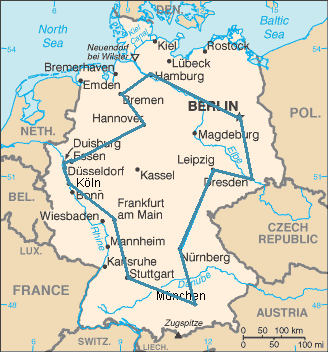
\includegraphics[width=0.5\linewidth]{lection_21/germany}
	\caption{Оптимальный маршрут коммивояжёра через 15 крупнейших городов Германии}
	\label{ris1}
\end{figure}

Таким образом оптимизировать эту задачу невозможно.

%рис 3, нужно доехать из A в B и посетить все пункты
\subsection{Задача о китайском почтальоне}
%рис 4
\textbf{Задача:} \emph{пройти по каждому ребру графа минимум 1 раз, чтобы доставить почту. Требуется найти такой цикл минимального суммарного веса.}

То есть, нам необходимо найти цикл минимального суммарного веса, такой, что он проходит по ребру хотя бы 1 раз. Важное замечание --- если граф Эйлеров, то Эйлеров цикл и есть решение этой задачи. А вот если его нет, то задача усложняется --- решение можно найти только полным перебором. Итоговый алгоритм получается неэффективным, т.к. его асимптотика $O(N!)$.
\chapter{Деревья. Двоичное дерево поиска.}
\section{Двоичное дерево. Класс  дерево.}
\textsf{k-ичное дерево} --- дерево, в котором количество дочерних вершин у каждой вершины не больше k штук. При этом троичное дерево является одновременно и четверичным --- просто четвертого ребра еще нет. Последовательность дочерних вершин может быть неупорядоченной. Нам же интересен случай, когда k-ичное дерево является упорядоченным. 

Рассмотрим двоичное дерево, упорядоченное, в общем случае не сбалансированное (в отличии от кучи). Двоичное дерево можно нарисовать так, что мы будем называть дочерние вершины "левая"\ или "правая" (по аналогии с кучей). 

\textsf{Поддерево} (правое/левое) --- подграф дерева, корень которого является дочерней вершиной (правой/левой). 

В прошлом семестре вводился такой способ хранения данных как односвязный список. Оказывается, можно реализовать такое звено, которое подходит для двоичного дерева поиска. Сделаем 2 указателя: на левое поддерево и правое поддерево, также указатель наверх (т.е. на родителя). Из таких звеньев можно собирать дерево.

Удобно считать пустой граф пустым деревом (хотя по определению дерева это неверно).

\begin{infa}{Класс Дерево}
\ \num \classi Node:
\ \num \tab \defi __init__(self, key, value): \com{Создаем звено ключ, значение}
\ \num \tab \tab self.key = key 
\ \num \tab \tab self.value = value 
\ \num \tab \tab self.parent = \Nonei
\ \num \tab \tab self.left = \Nonei
\ \num \tab \tab self.right = \Nonei
\ \num
\ \num \classi Tree:
\num \tab \defi __init__(self):
\num \tab \tab self.root = \Nonei
\num \tab \defi print(self, node):
\num \tab \tab \ifi node \isi \Nonei: \com{Благодаря этому нам не важно, пустое наше поддерево\\\phantom{ 5\ \ \ \ } или нет - крайний случай проверен}
\num \tab \tab \tab \returni
\num \tab \tab self.print(node.left)
\num \tab \tab \printi((node.key, node.value)) \com{Это не совсем обратный ход рекурсии}
\num \tab \tab self.print(node.right)
\end{infa}

\section{Двоичное дерево поиска}
\textsf{Двоичное дерево поиска} --- это корневое двоичное упорядоченное дерево, построенное по следующему правилу для любого звена node: все ключи левого поддерева $key_i<key_{node}$, все ключи правого поддерева $key_j>key_{node}$.

Возьмем такие числа:
$$
6\ 3\ 5\ 4\ 2\ 9\ 7\ 8\ 1\ 11\ 10\ 12\ 0
$$
и изобразим для них двоичное дерево поиска (рис. \ref{fig_dvderevo}).

\begin{figure}
	\centering
	%\vspace{-2.5cm}
	\def\svgwidth{17cm} % если надо изменить размер
	\input{lection_22/graph_derevo.pdf_tex}
	\caption{Двоичное дерево поиска}
	\label{fig_dvderevo}
	%\vspace{-9cm}
\end{figure}

Алгоритм построения: сначала дерево пустое и ни одного звена нет. Берем числа поочереди. 3 меньше 6, поэтому 6 становится главной. 3 становится левым поддеревом шестерки, т.к. $3<6$ (добавляем числа меньшие корня в левое поддерево, а числа большие корня в правое поддерево). Далее число 5 меньше 5, но больше 3. Поэтому 5 находится в левом поддереве 6, но в правом поддереве тройки. Дальнейшее построение аналогично. Красота такого метода в том, что если <<спроектировать>> числа на прямую, получается числовая ось, на которой числа расставлены в порядке возрастания.

Двоичное дерево поиска работает как бинарный поиск. Количество операций сравнения равно высоте дерева $O(\log_2N)$ (если дерево сбалансировано). Чем оно лучше бинарного поиска в списке? Для добавления элемента требуется то же время ($O(\log_2N)$). Но в списке после того, как мы нашли, куда вставить элемент, требуется сделать циклический сдвиг.

Если у элемента нет дочерних вершин, а его надо удалить, то это сделать просто. Но вот если у него есть одна дочерняя вершина, мы присоединяем оставшееся дерево к верхнему родителю (можно привести аналогию с подчиненными: если начальника подчиненных уволили, то эти подчиненные становятся подчиненными начальника рангом выше).

В случае когда нужно присоеденить 2 дерева (т.е. если мы удалили вершину, у которого было 2 поддерева, например третью) переходим к левому поддереву удаляемой вершины и к самому правому из него добавляем правое поддерево той вершины, которую мы удалили. Минусы: при удалении корневого элемента длина дерева удваивается.

Но есть более оптимальный вариант: после удаления вершины (например тройки) возьмем самый правый элемент левого поддерева этой вершины (т.е. тройки) и поставим его вместо элемента, которого мы удалили (т.е. вместо стройки), что предотвратит от удваивания длины всего дерева (т.е. если бы у двойки было бы правое поддерево, мы бы нашли самый большой элемент в этом поддереве и поставили бы его на место тройки).

Почему не воспользоваться хеш--таблицей? Хеш--таблица не упорядочена, в отличии от двоичного дерева поиска.
\chapter{Двоичное дерево поиска. Продолжение.}
\section{Класс Дерево. Продолжение.}
%Будет разумным погрузить класс звена в дерево
\begin{infa}{Класс Дерево}
\ \num \classi Tree:
\ \num \tab \classi Node: \com{Класс в классе можно делать, т.к. в классе описано свое\\\phantom{12\ \ \ \ \ \ \ } пространство имен}
\ \num \tab \tab \defi __init__(self, data):
\ \num \tab \tab \tab self.parent = \Nonei
\ \num \tab \tab \tab self.left = \Nonei
\ \num \tab \tab \tab self.right = \Nonei
\ \num \tab \tab \tab self.key = data
\ \num \tab \defi __init__(self):
\ \num \tab \tab self.root = \Nonei
\num \tab \defi find(self, data):
\num \tab \tab p = self.root
\num \tab \tab \whilei p \isi \noti \Nonei \andi p.key != data: \com{Важна последовательность\\\phantom{12\ \ \ \ \ \ \ } написаний условий, т.к. может быть ошибка при проверке ключа}
\num \tab \tab \tab \ifi data > p.key:
\num \tab \tab \tab \tab p = p.right
\num \tab \tab \tab \elsei:
\num \tab \tab \tab \tab p = p.left
\num \tab \tab \returni p
\num \tab \defi insert(self, data):
\num \tab \tab p = self.find(data) \com{Одно и то же число не может храниться дважды, \\\phantom{12\ \ \ \ \ \ \ }как в множестве, но значения могут повторяться}
\num \tab \tab \ifi p \isi \noti \Nonei:
\num \tab \tab \tab \returni
\num \tab \tab node = Tree.Node(data)
\num \tab \tab \ifi self.root \isi \Nonei:
\num \tab \tab \tab self.root = node
\num \tab \tab \tab \returni
\num \tab \tab p = self.root
\num \tab \tab \whilei \Truei:
\num \tab \tab \tab \ifi data < p.key:
\num \tab \tab \tab \tab \ifi p.left \isi \Nonei:
\num \tab \tab \tab \tab \tab p.left = node
\num \tab \tab \tab \tab \tab node.parent = p
\num \tab \tab \tab \tab \tab \breaki
\num \tab \tab \tab \tab \elsei:
\num \tab \tab \tab \tab \tab p = p.left 
\num \tab \tab \tab \elsei:
\num \tab \tab \tab \tab \ifi p.right \isi \Nonei:
\num \tab \tab \tab \tab \tab p.right = node
\num \tab \tab \tab \tab \tab node.parent = p
\num \tab \tab \tab \tab \tab \breaki
\num \tab \tab \tab \tab \elsei:
\num \tab \tab \tab \tab \tab p = p.right
\end{infa}
\section{Балансировка дерева}
Двоичное дерево поиска \textsf{сбалансированно}, если для каждой его вершины высота левого и правого поддерева отличаются не более чем на единицу.
	
%нарисуем закошеное дерево 
\textbf{Инвариант}: та вершина, которая левее других вершин, должна остаться левее всех вершин, т.е двигать вверх--вниз вершины можно, но влево--вправо двигать нельзя, иначе нарушится последовательность чисел.

Алгоритм балансировки подробно описан в \href{https://ru.wikipedia.org/wiki/%D0%90%D0%92%D0%9B-%D0%B4%D0%B5%D1%80%D0%B5%D0%B2%D0%BE#.D0.91.D0.B0.D0.BB.D0.B0.D0.BD.D1.81.D0.B8.D1.80.D0.BE.D0.B2.D0.BA.D0.B0}{википедии}.

\textsf{АВЛ--дерево} --- сбалансированное по высоте двоичное дерево поиска: для каждой его вершины высота её двух поддеревьев различается не более чем на 1.


\textsf{Красно--чёрное дерево} --- это одно из самобалансирующихся двоичных деревьев поиска, гарантирующих логарифмический рост высоты дерева от числа узлов и быстро выполняющее основные операции дерева поиска: добавление, удаление и поиск узла. Сбалансированность достигается за счёт введения дополнительного атрибута узла дерева --- «цвета». Этот атрибут может принимать одно из двух возможных значений --- «чёрный» или «красный».

\textbf{Свойства} красно--черного дерева:
\begin{enumerate}
	\item Узел либо красный, либо чёрный.
	\item Корень --- чёрный. (В других определениях это правило иногда опускается. Это правило слабо влияет на анализ, так как корень всегда может быть изменен с красного на чёрный, но не обязательно наоборот).
	\item Все листья --- чёрные.
	\item Оба потомка каждого красного узла --- чёрные.
	\item Всякий простой путь от данного узла до любого листового узла, являющегося его потомком, содержит одинаковое число чёрных узлов.
\end{enumerate}

\chapter{Кодирование}
\section{Равномерное и неравномерное кодирование}
Есть два глобальных подхода в кодировании текста: равномерное кодирование и неравномерное кодирование.

Обозначим алфавит допустимых символов $\mathbb{A}$.

В неравномерном кодировании код символов разной длины (например, UNICODE UTF 8 --- одна из
самых популярных кодировок).

Рассмотрим четырехбуквенное кодирование. Закодируем буквы <<А>>, <<Б>>, <<В>>, <<Г>> таким образом:
\begin{center}
	$
\begin{array}{rl}
\text{А} &= 0\\
\text{Б} &= 1\\
\text{В} &= 10\\
\text{Г} &= 111\\
\end{array}
$
\end{center}
Тогда запись <<ГАГА>> можно закодировать так:
\begin{center}
ГАГА = 11101110 = БББГА,
\end{center}
т.е. декодирование неоднозначно, такое кодирование плохое.

\textbf{Условие Фано:} \textit{для того, чтобы сообщение, записанное с помощью неравномерного по длине кода, однозначно раскодировалось, достаточно, чтобы никакой код не был началом другого (более длинного) кода.} \textbf{Обратное условие Фано} (\textit{ни один код не является концом (суффиксом) другого}) также является достаточным условием однозначного декодирования неравномерного кода.

Тогда пусть
\begin{center}
$
\begin{array}{rl}
\centering
\text{А} &= 0\\
\text{Б} &= 110\\
\text{В} &= 10\\
\text{Г} &= 111\\
\end{array}
$
\end{center}

Возьмем (для удобства рядом записан столбец в зеркальном отражении):
\begin{center}
$
\begin{array}{rlcr}
\text{A} = &1&\vrule&1\\
\text{Б} = &10&\vrule&01\\
\text{В} = &100&\vrule&001\\
\text{Г} = &000&\vrule&000\\
\end{array}
$
\end{center}
Тогда
\begin{center}
БАГАВА = 10100011001 
\end{center}
--- 1100 нет, т.е в конце ВА. 1000 тоже нет, т.е. по середине ГА. 101 нет, в начале БА. Однозначность есть, хотя и декодировать очень сложно. 

Составим суффиксное дерево. Оно не нужно при декодировании, а при доработке дерева (дополнении алфавита) является полезным инструментом. Способ составления: отзеркаливаем код и строим дерево, в котором каждое ребро --- цифра в коде.

Кодировка в равномерном кодировании UTF-16. Можно закодировать $2^n$ различных символов (мощность алфавита).
%FIXME вставить рисунок префиксного дерева

\section{Поиск подстроки в строке}
\subsection{Наивный поиск подстроки в строке}
\begin{infa}{Примитивный поиск подстроки в строке}
\ \num s = "abbbbabbaaabbababaabb"
\ \num subs = "bbbaba"
\ \num \defi find(s, sub):
\ \num \tab \fori pos \ini \rangei(0, \leni(s)-\leni(sub)+1):
\ \num \tab \tab \fori i \ini \rangei(\leni(sub)):
\ \num \tab \tab \tab \ifi sub[i] != s[pos+i]:
\ \num \tab \tab \tab \tab \breaki
\ \num \tab \tab \elsei:
\ \num \tab \tab \tab \returni pos
\num \tab \returni -1
\end{infa}
Построчный комментарий кода:\\
4) Имеет смысл проходить по основной строке, пока входящая строка влезает в рассматриваемый участок.\\
5)--6) Пробегаемся по элементам входящей строки и смотрим, совпадают ли они с элементами основной.\\
7) Если нет, уже можно переходить к следующему элементу основной строки.\\
9) Если прошли по всем элементам строки вхождения, можно выдать ту позицию, начиная с которой есть вхождение.\\
10) Если вхождения нет, выдается ‘-1’.

Сложность алгоритма $O(N\cdot M)$. В итоге алгоритм получается неэффективным.
\subsection{Конечный автомат поиска <<abcd>>}
Смотрим на каждый символ только  по одному разу! Методика хранения автомата: орграф. Если конечный автомат уже построен, то время поиска $O(N)$, $N$ --- длина строки.

Конечный автомат поиска является частным случаем машины Тьюринга, Подход таков:
\begin{enumerate}
	\item Изначально система в фазе ноль.
	\item Сравниваем букву в основной строке с буквой во входящей строке. Если они совпали, то код продвигается на фазу вперед.
	\item Сравниваем следующие буквы. Если они совпали, переходим в фазу два и т.д.
	\item В случае несовпадения фаза становится нулевой.
\end{enumerate}

\begin{infa}{Конечный автомат для поиска подстроки <<abcd>>}
\ \num state = 0
\ \num \fori c in s:
\ \num \tab \ifi state == 0:
\ \num \tab \tab \ifi c == "a":
\ \num \tab \tab \tab state = 1
\ \num \tab \elifi state == 1:
\ \num \tab \tab \ifi c == 'b':
\ \num \tab \tab \tab state = 2
\ \num \tab \tab \elifi c == 'a':
\num \tab \tab \tab state = 1
\num \tab \tab \elsei:
\num \tab \tab \tab state = 0
\num \tab \elifi state == 2:
\num \tab \tab \ifi c == 'c':
\num \tab \tab \tab state = 3
\num \tab \tab \elifi c == 'a':
\num \tab \tab \tab state = 1
\num \tab \tab \elsei:
\num \tab \tab \tab state = 0
\num \tab \elifi state == 3:
\num \tab \tab \ifi c == 'a':
\num \tab \tab \tab state = 1
\num \tab \tab \elifi c == 'd':
\num \tab \tab \tab state = 4
\num \tab \tab \elsei:
\num \tab \tab \tab state = 0
\end{infa}
\section{Расстояние Левенштейна}
\subsection{Определение}
\textbf{Расстояние Левенштейна} (также редакционное расстояние или дистанция редактирования) \textbf{между двумя строками в теории информации и компьютерной лингвистике} --- \textit{это минимальное количество операций вставки одного символа, удаления одного символа и замены одного символа на другой, необходимых для превращения одной строки в другую.}

Есть 2 строки Мама и Мим. Мы можем превратить их друг в друга путем вставки символа, удаления символа. Минимальный путь в данном случае --- удаление последнего и замена, т.е. длина пути 2. Так и определяется расстояние Левенштейна.

a[:i], b[:j] --- срезы до i--го и j--го символа.
$F_{ij} = L(a[:i], b[:j])$ --- расстояние Левенштейна. Тогда\\
$$F_{ij}=
\begin{cases}
\text{Последниие буквы совпадают, то } F_{(i-1)(j-1)}\\
1+\min(F_{(i-1)(j-1)}, F_{(i-1)j}, F_{i(j-1)})
\end{cases}
$$
\subsection{Реализация алгоритма поиска расстояния Левенштейна}
\begin{infa}{Рекуррентная реализация поиска расстояния Левенштейна}
\num \defi lev(a, b):
\num \tab \ifi \noti a: 
\num \tab \tab \returni \leni(b)
\num \tab \ifi \noti b: 
\num \tab \tab \returni \leni(a)
\num \tab \returni \mini(lev(a[1:], b[1:])+(a[0] != b[0]), lev(a[1:], b)+1, lev(a, b[1:])+1)
\end{infa}
Данный алгоритм записывается компактно, но асимптотика этого алгоритма ужасна.

\begin{infa}{Реализация поиска расстояния Левенштейна}
\ \num \defi levenshtein(s1, s2):
\ \num \tab \ifi \leni(s1) < \leni(s2):
\ \num \tab \tab \returni levenshtein(s2, s1)
\ \num 
\ \num \tab \ifi \leni(s2) == 0:
\ \num \tab \tab \returni \leni(s1)
\ \num
\ \num \tab previous_row = \rangei(\leni(s2) + 1)
\ \num \tab \fori i, c1 \ini \enumeratei(s1):
\num \tab \tab current_row = [i + 1]
\num \tab \tab \fori j, c2 \ini \enumeratei(s2):
\num \tab \tab \tab insertions = previous_row[j + 1] + 1
\num \tab \tab \tab deletions = current_row[j] + 1     
\num \tab \tab \tab substitutions = previous_row[j] + (c1 != c2)
\num \tab \tab \tab current_row.append(\mini(insertions, deletions, substitutions))
\num \tab \tab previous_row = current_row
\num
\num \tab \returni previous_row[-1]
\end{infa}
\chapter{Z--функция строки и ее вычисление}
Основной материал лекции взят с \href{http://e-maxx.ru/algo/z_function}{сайта}.
\section{Z--функция}
\subsection{Определение}
Пусть дана строка $s$ длины $n$. Тогда Z--функция от этой строки --- это массив длины $n$, i-ый элемент которого равен наибольшему числу символов, начиная с позиции i, совпадающих с первыми символами строки $s$.

Иными словами, \texttt{z[i]} -- это наибольший общий префикс строки $s$ и её i--го суффикса.

Во избежание неопределённости, мы будем считать строку 0--индексированной --- т.е. первый символ строки имеет индекс 0, а последний --- $n-1$.

Первый элемент Z--функции, \texttt{z[0]}, обычно считают неопределённым. Мы будем считать, что он равен нулю.

\subsection{Реализация}
\subsubsection{Тривиальный алгоритм}
\begin{infa}{Тривиальный алгоритм}
\num \defi z_function_trivial(s):
\num \tab n = \leni(s)
\num \tab z = [0]*n
\num \tab i = 1
\num \tab \whilei i < n:
\num \tab  \tab \whilei i + z[i] < n \andi s[z[i]] == s[i+z[i]]: \com{Пока мы не дошли до\\\phantom{3\ \ \ \ \ \ \ } конца и символ на позиции z[i] равен символу на рассматриваемой позиции + z[i]\\\phantom{3\ \ \ \ \ \ \ } (т.е., это и есть основная проверка)}
\num \tab \tab \tab z[i] += 1
\num \tab \tab i += 1
\num \tab \returni z
\end{infa}
Сложность такого алгоритма $O(N^2)$. 

\subsubsection{Эффективный алгоритм}
Чтобы получить эффективный алгоритм, будем вычислять значения \texttt{z[i]} по очереди — от i=1 до $n-1$, и при этом постараемся при вычислении очередного значения \texttt{z[i]} максимально использовать уже вычисленные значения.
\begin{infa}{Эффективная реализация Z--функции}
\ \num \defi z_function(s):
\ \num \tab z = [0]*\leni(s)
\ \num \tab left = 0  
\ \num \tab right = 0
\ \num \tab x = 0
\ \num \tab \fori i \ini \rangei(1, \leni(s)):
\ \num \tab \tab \ifi i <= right:
\ \num \tab \tab \tab x = \mini(z[i-left], right - i + 1)
\ \num \tab \tab \elsei:
\num \tab \tab \tab x = 0 
\num \tab \tab \whilei i+x < \leni(s) \andi s[x] == s[i+x]:
\num \tab \tab \tab x += 1
\num \tab \tab \ifi i + x - 1  > right:
\num \tab \tab \tab left, right = i, i + x - 1
\num \tab \tab z[i] = x
\num \tab \returni z
\end{infa}
Этот алгоритм выполняется за линейное время.

\subsection{Применение}
Применения Z--функции:
\begin{itemize}
	\item Поиск подстроки в строке.
	\item Поиск количества различных подстрок в строке.
	\item Сжатие строки.
\end{itemize}

Запишем реализацию поиска количества различных подстрок в строке.
\begin{infa}{Поиск количества различных подстрок в строке}
\ \num \defi count_different_substrings(s):
\ \num \tab n = \leni(s)
\ \num \tab start = s[0]
\ \num \tab res = 0
\ \num \tab \fori i \ini \rangei(1, n):
\ \num \tab \tab t = start[::-1]
\ \num \tab \tab k = \leni(t) - \maxi(z_function(t))
\ \num \tab \tab res += k
\ \num \tab \tab start += s[i]
\num \tab \returni res
\end{infa}
\chapter{Z и префикс функция строки}
\section{Z--функция строки}
Z--функция строки --- функция от номера символа.
Z--функция --- это массив длинны \texttt{len(S) = N}, \texttt{z[i]} --- длина совпадающего префикса у строки \texttt{S} и \texttt{S[i:]}.

\texttt{z[0]} не определено. Но мы будем считать, что \texttt{z[0] = 0}. 

\begin{center}
"a a a a a"\\
z=[0, 4, 3, 2, 1]\\

"a b a c a b a"\\
z=[0, 0, 1, 0, 3, 0]
\end{center}

Зачем нужна z--функция?
Будем искать строчку \texttt{p=aba} и все ее вхождения в строке \texttt{abacabadabacaba}. Склеим две строки символом, которого точно нет ни там ни там:
\begin{center}
	\texttt{s = "aba\#abacabadabacaba"}.
\end{center}
Т.к. стоит символ \#, длина искомой подстроки не может быть больше 3.
$$
z = [0, 0, 1, 0, 3, 0, 1, 0, 3, 0, 1, 0, 3, 0, 1, 0, 3, 0, 1]
$$
Там, где \texttt{z[i] == len(p)}, т.е. там, где величина Z--функции равна длине подстроки, у нас есть совпадение, т.е. там подстрока содержится в строке. Позиция вхождения: найдена подстрока в строке, \texttt{pos = i-len(p)-1} --- номер вхождения.

Тривиальное вычисление Z--функции (требует $O(N^2)$).
\begin{infa}{Тривиальное вычисление Z--функции}
\num N = \leni(s)
\num z=[0]
\num left = right = 0
\num \fori i \ini \rangei(1, N):
\num \tab x = 0
\num \tab \whilei i + x < N \andi s[x] == s[i+x]:
\num \tab \tab x += 1
\num \tab z[i] = x
\num \tab if i + x - 1> right: \com{Сохраянем z--блок}
\num \tab \tab left, right = i, i + x - 1
\end{infa}
z--блок --- срез строки \texttt{s[i:i+z[i]]}, т.е. это часть строки, совпавшая с подстрокой.

На момент вычисления \texttt{z[i]} существует самый правый отрезок совпадения. Длина этого отрезка равна разнице его правого и левого конца + 1.

\begin{infa}{}
	\ \num N = \leni(s)
	\ \num z=[0]
	\ \num left = right = 0
	\ \num \fori i \ini \rangei(1, N):
	\ \num \tab x = \mini(z[i-left], right - i + 1) \ifi i<=right \elsei 0
	\ \num \tab \whilei i + x < N \andi s[x] == s[i+x]:
	\ \num \tab \tab x += 1
	\ \num \tab z[i] = x
	\ \num \tab \ifi i + x - 1> right: \com{Сохраянем z--блок}
	\num \tab \tab left, right = i, i + x - 1
\end{infa}
Этот алгоритм работает за линейное время.
\section{Префикс--функция строки. Алгоритм Кнута — Морриса — Пратта.}
\subsection{Префикс--функция строки}
Собственным суффиксом строки называется суффикс, не совпадающий со всей строкой, совпадающий с ее префиксом. 

Префикс--функция строки \texttt{$\pi$[i]} --- массив длинной строки, где \texttt{$\pi$[i]} --- длина наибольшего по длине собственного суффикса подстроки (среза) \texttt{s} начиная от начала и до позиции \texttt{i (s[:i+1])}.
\begin{center}
"a a a a a"\\
pi=[0, 1, 2, 3, 4]\\
"a b a c a b a"\\
pi = [0, 0, 1, 0, 1, 2, 3]\\
\end{center}
Заметим, что эта функция всегда растет на единицу.
\begin{infa}{Тривиальный алгоритм}
\num N = \leni(s)
\num pi = [0]*N
\num \fori i \ini \rangei(1, N):
\num \tab \fori k \ini \rangei(i+1):
\num \tab \tab \ifi s[0:k] == s[i-k+1:i+1]:
\num \tab \tab \tab pi[i] = k
\end{infa}
Асимптотика $O(N^3)$.

\begin{infa}{Эффективный алгоритм}
\num \defi prefix(s):
\num \tab n = \leni(s)
\num \tab pi = [0]*n
\num \tab \fori i \ini \rangei(1, n):
\num \tab \tab j = pi[i-1]
\num \tab \tab \whilei j > 0 \andi s[i] != s[j]:
\num \tab \tab \tab j = pi[j-1]
\num \tab \tab \ifi s[i] == s[j]:
\num \tab \tab \tab j += 1
\num \tab \tab pi[i] = j
\num \tab \returni pi
\end{infa}

\subsection{Поиск подстроки в строке}
Эта задача является классическим применением префикс-функции (и, собственно, она и была открыта в связи с этим).

Дан текст t и строка s, требуется найти и вывести позиции всех вхождений строки s в текст t.

Обозначим для удобства через n длину строки s, а через m — длину текста t.

Образуем строку s + \# + t, где символ \# — это разделитель, который не должен нигде более встречаться. Посчитаем для этой строки префикс-функцию. Теперь рассмотрим её значения, кроме первых n+1 (которые, как видно, относятся к строке s и разделителю). По определению, значение $\pi$[i] показывает наидлиннейшую длину подстроки, оканчивающейся в позиции i и совпадающего с префиксом. Но в нашем случае это $\pi$[i] — фактически длина наибольшего блока совпадения со строкой s и оканчивающегося в позиции i. Больше, чем n, эта длина быть не может — за счёт разделителя. А вот равенство $\pi$[i] = n (там, где оно достигается), означает, что в позиции i оканчивается искомое вхождение строки s (только не надо забывать, что все позиции отсчитываются в склеенной строке s+\#+t).

Таким образом, если в какой-то позиции i оказалось $\pi$[i] = n, то в позиции i - (n + 1) - n + 1 = i - 2 n строки t начинается очередное вхождение строки s в строку t.

Как уже упоминалось при описании алгоритма вычисления префикс-функции, если известно, что значения префикс-функции не будут превышать некоторой величины, то достаточно хранить не всю строку и префикс-функцию, а только её начало. В нашем случае это означает, что нужно хранить в памяти лишь строку s + \# и значение префикс-функции на ней, а потом уже считывать по одному символу строку t и пересчитывать текущее значение префикс-функции.

Итак, алгоритм Кнута-Морриса-Пратта решает эту задачу за O(n+m) времени и O(n) памяти.

Подробнее материал лекции изложен на \href{http://e-maxx.ru/algo/prefix_function}{сайте}.
\chapter{Автоматы}
\section{Машина Тьюринга}
Это абстрактный исполнитель, живущий на бесконечной ленте, в клетках которой находятся буквы $\alpha$ принадлежащие фиксированному алфавиту A. Каретка машины Тьюринга может двигаться по ленте влево или вправо. Каретка может видеть, что нарисовано на ленте (на текущей клетке). Также у нее есть возможность изменять символы на ленте, т.е. она может записать, изменить. А также у нее есть состояние q. При этом это состояние принадлежит множеству допустимых состояний Q. Подмножество состояний --- состояние останова (остановки). Это подмножество конечно. Поведение этой машины детерминированно (оно задается увиденным символом и предыдущим состоянием). Она из исходного состояния переходит в новое состояние, в котором определено: 1) Состояние системы 2) Считанный символ 3) Действие.

Множества Q и A конечные. Возможно очень большие, но конечные. Мощность множества --- число конечных состояний в нем.

Программа, которую мы написали, не хранится нигде. Типа в памяти каретки. Нужно её куда--то записать. Самое простое --- написать не ленте. Тогда каретка, которая едет на двух лентах сразу --- универсальная (программируемая) машина Тьюринга. О скорости работы нет разговора. Есть вопрос о вычислимости алгоритма.
\section{Вычислимость функций (алгоритмов)}
Что по сути такое алгоритм? Есть определенные возможные входные данные. Есть множество значений --- множество возможных результатов. Алгоритм --- своего рода функция, которая переводит множество определения в множество значений. Но невычислимые функции. Вычислимые функции (алгоритмы) --- это алгоритмы. Функции называются вычислимыми, если есть возможность посчитать её через машину Тьюринга. То, что мы называем раличными алгоритмами (все виды сортировок) --- это, с точки зрения вычислимости - один алгоритм. Нам ведь не важен путь (как и не важна скорость). Нам важно, что есть возможность получить результат, не более того. А какие алгоритмы невычислимые? Например, доказано, что нельзя вычислить вычислимость программы. Т.е. невозможно написать программу, которая посчитает, закончится программа или нет.

Исполнители А и В называются алгоритмически эквивалентными, если можно сэмулировать А на В и В на А.

\section{Клеточные автоматы. Игра жизнь Джона Конвая}
Простейшие автоматы --- это клетки, живущие не линии. В клетках --- нули и единицы. Состояние клетки зависит только от самой клетки и от двух ее ближайших соседей. В каждый следующий момент времени клетка меняет свое состояние в зависимости от своего и соседей состояний. При этом для всех клеток алгоритмы одинаковы. Всего есть 256 клеточных автоматов (возможных комбинаций для данных состояний триад клеток). Среди них есть и совсем простые. Интересны несколько из них. Одно --- правило 30, т.к. порождает случайные хаотические структуры. Также есть правила жизни Джона Конвея. Если клетка была жива, то остается живой при 2 или 3 соседях. А если была мертва, то оживает при наличии трех соседей.


\end{document}